\section{Production}

The production of the position-sensitive device involves the necessary steps to produce the detector and arithmetic \gls{pcb}.

It's best to first do the arithmetic board and if it works, proceed with the detector.
Of course, if you only need one of the boards, perform the following steps only once.

\subsection{Commissioning}

% TODO: screenshots of HTML BOM files

Before we can assemble the \gls{pcb}s, we need to gather the required components and order missing pieces.

The list of the required components is usually known as the \gls{bom}.
You can generate a current \gls{bom} directly from \href{https://kicad-pcb.org}{KiCad} by using the \href{https://github.com/openscopeproject/InteractiveHtmlBom}{InteractiveHtmlBom} plugin.
The plugin generates an \gls{html} file that lists the components and their respective placement on the \gls{pcb}.
\Cref{fig:kicad_interactive_html_bom_plugin_menu} shows where to find the plugin in the \gls{pcb} editor menu.
You can check if the parts are stocked and placed.
\begin{figure}[H]
	\centering
	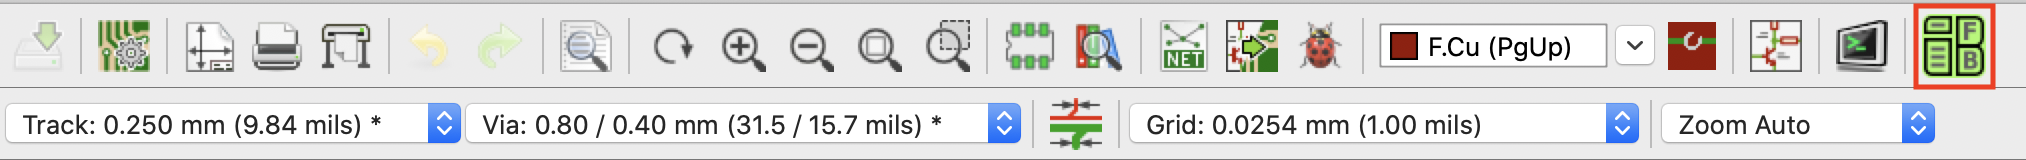
\includegraphics[scale=0.4]{screenshot/kicad_interactive_html_bom_plugin_menu}
	\caption{Menu entry for the \href{https://github.com/openscopeproject/InteractiveHtmlBom}{InteraciveHtmlBom} plugin for \href{https://kicad-pcb.org}{KiCad}}\label{fig:kicad_interactive_html_bom_plugin_menu}
\end{figure}
\Cref{fig:kicad_interactive_html_bom_plugin_arithmetic} and \cref{fig:kicad_interactive_html_bom_plugin_detector} show the view of the generated \gls{html} for the arithmetic and detector board.
\begin{figure}[H]
	\centering
	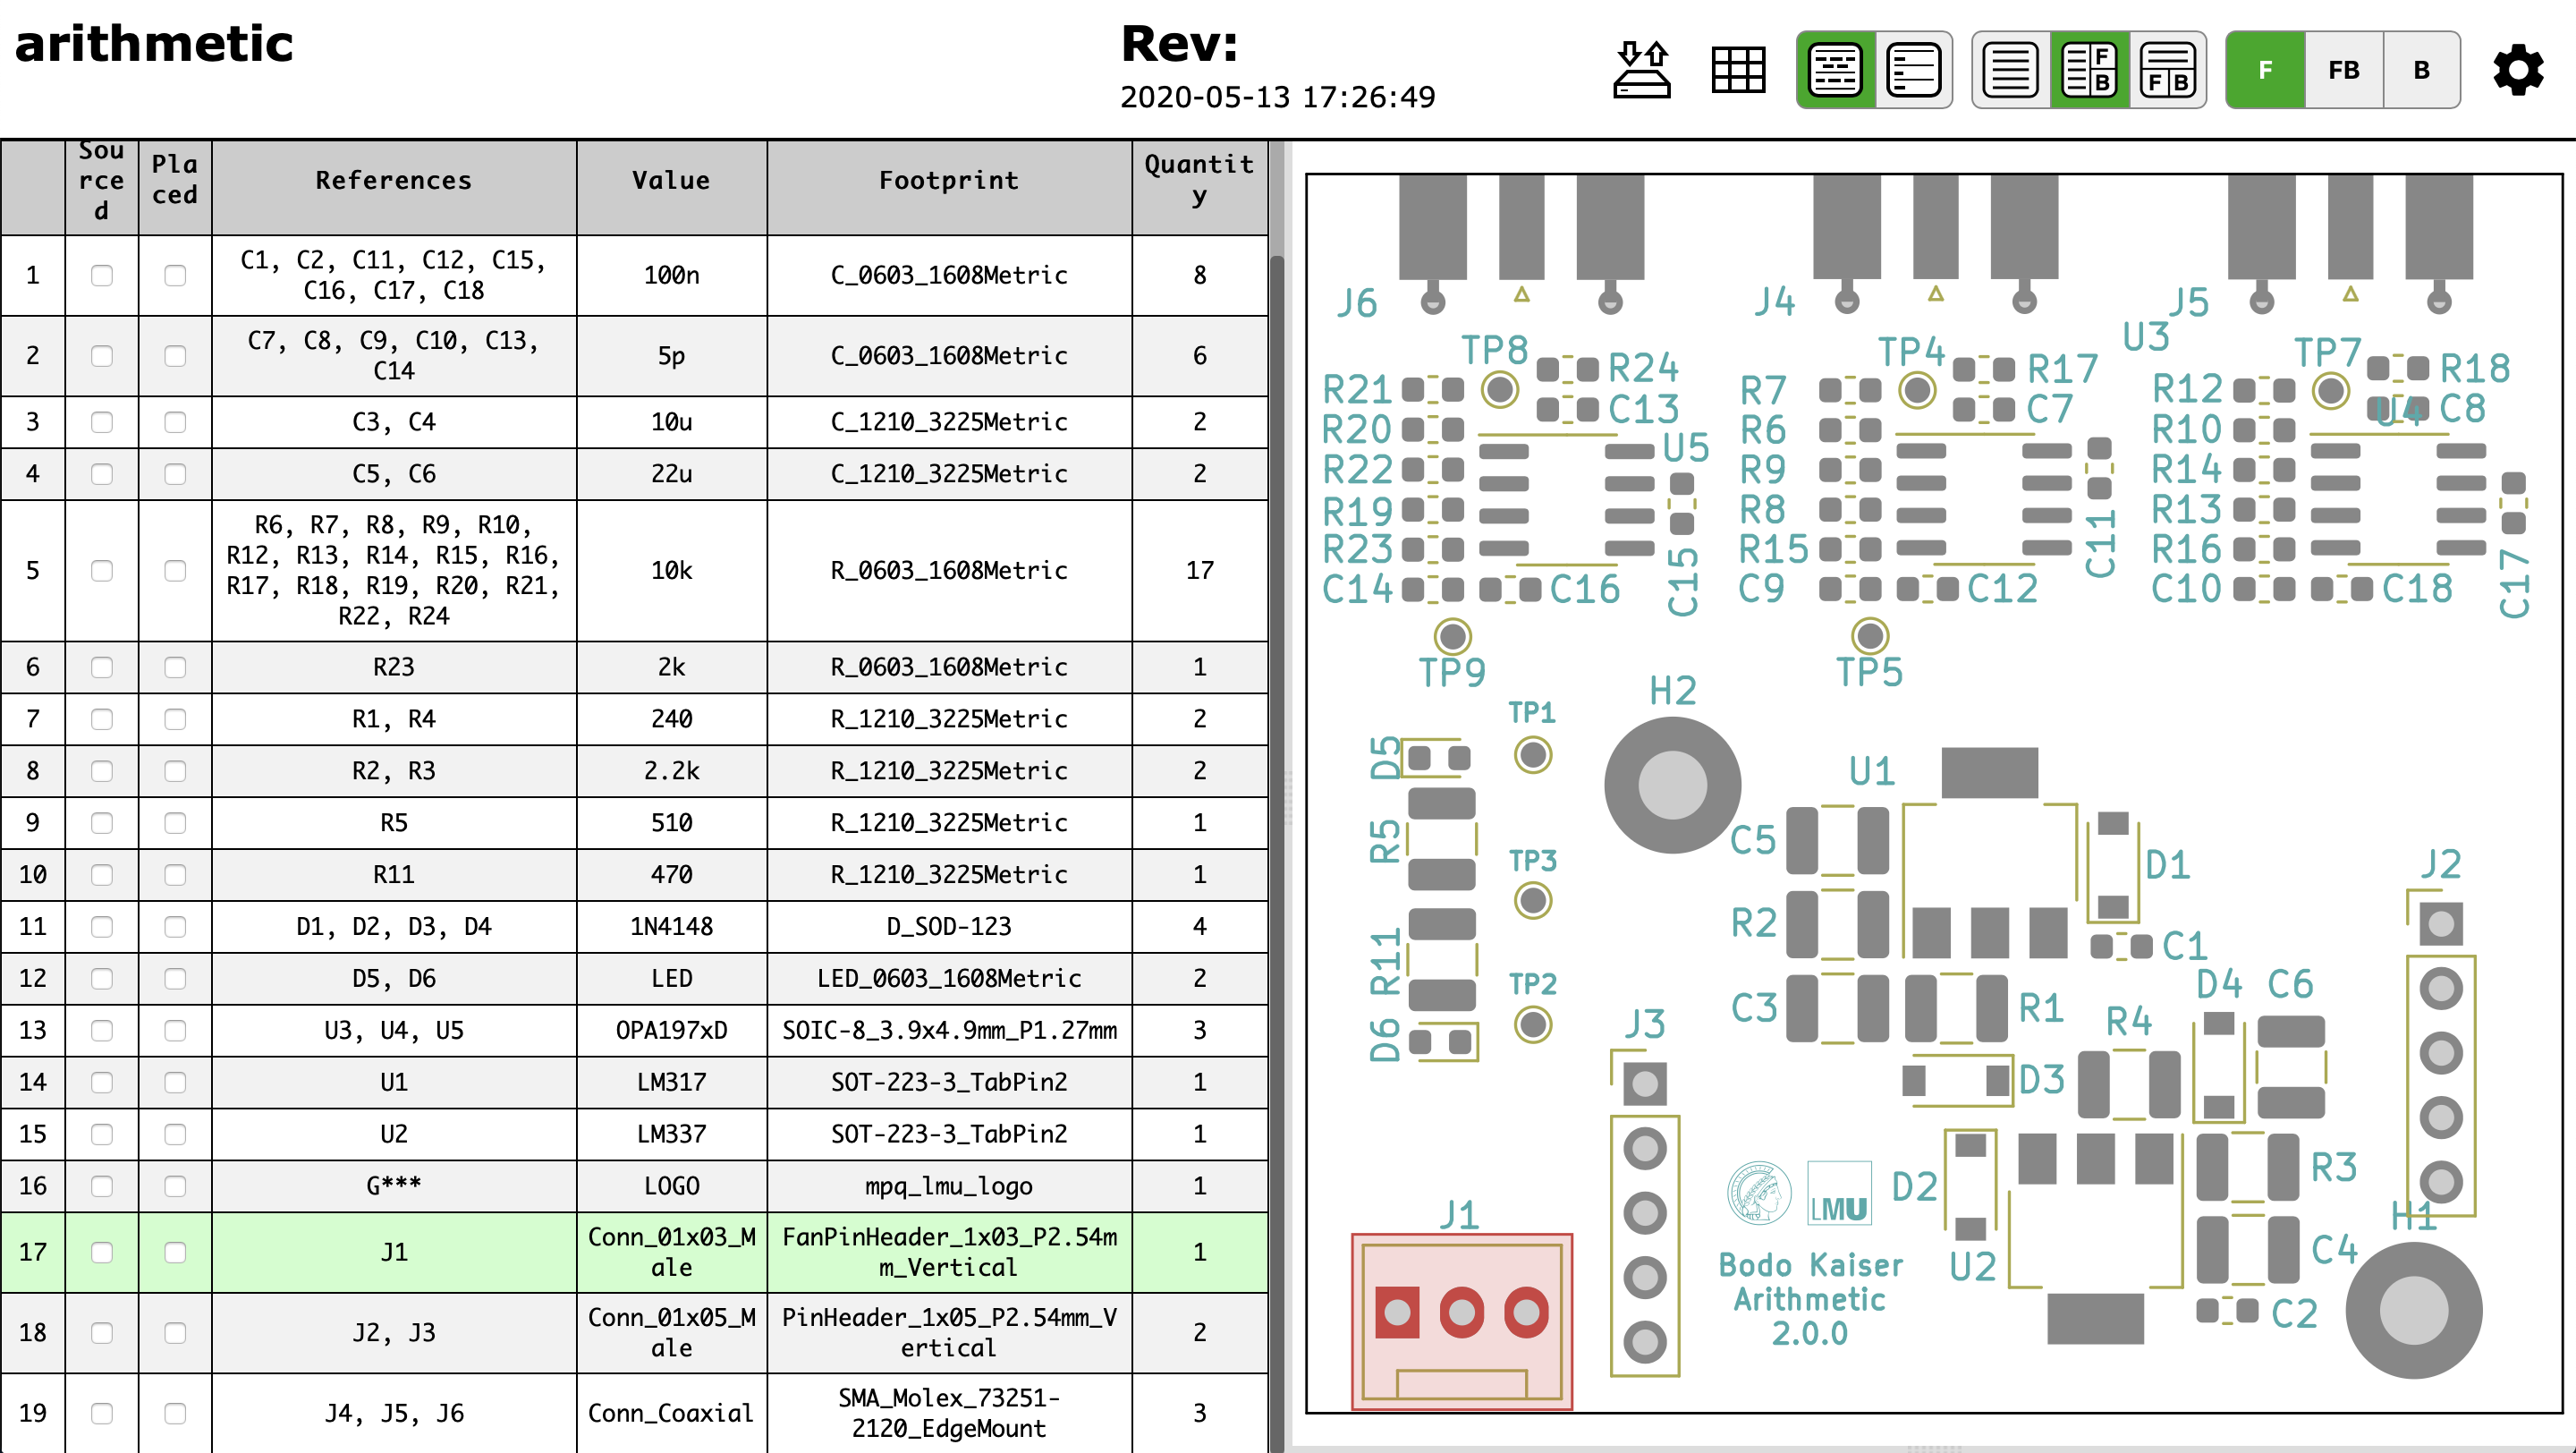
\includegraphics[scale=0.3]{screenshot/kicad_interactive_html_bom_plugin_arithmetic}
	\caption{Arithmetic board view of the \href{https://github.com/openscopeproject/InteractiveHtmlBom}{InteraciveHtmlBom} plugin}\label{fig:kicad_interactive_html_bom_plugin_arithmetic}
\end{figure}
\begin{figure}[H]
	\centering
	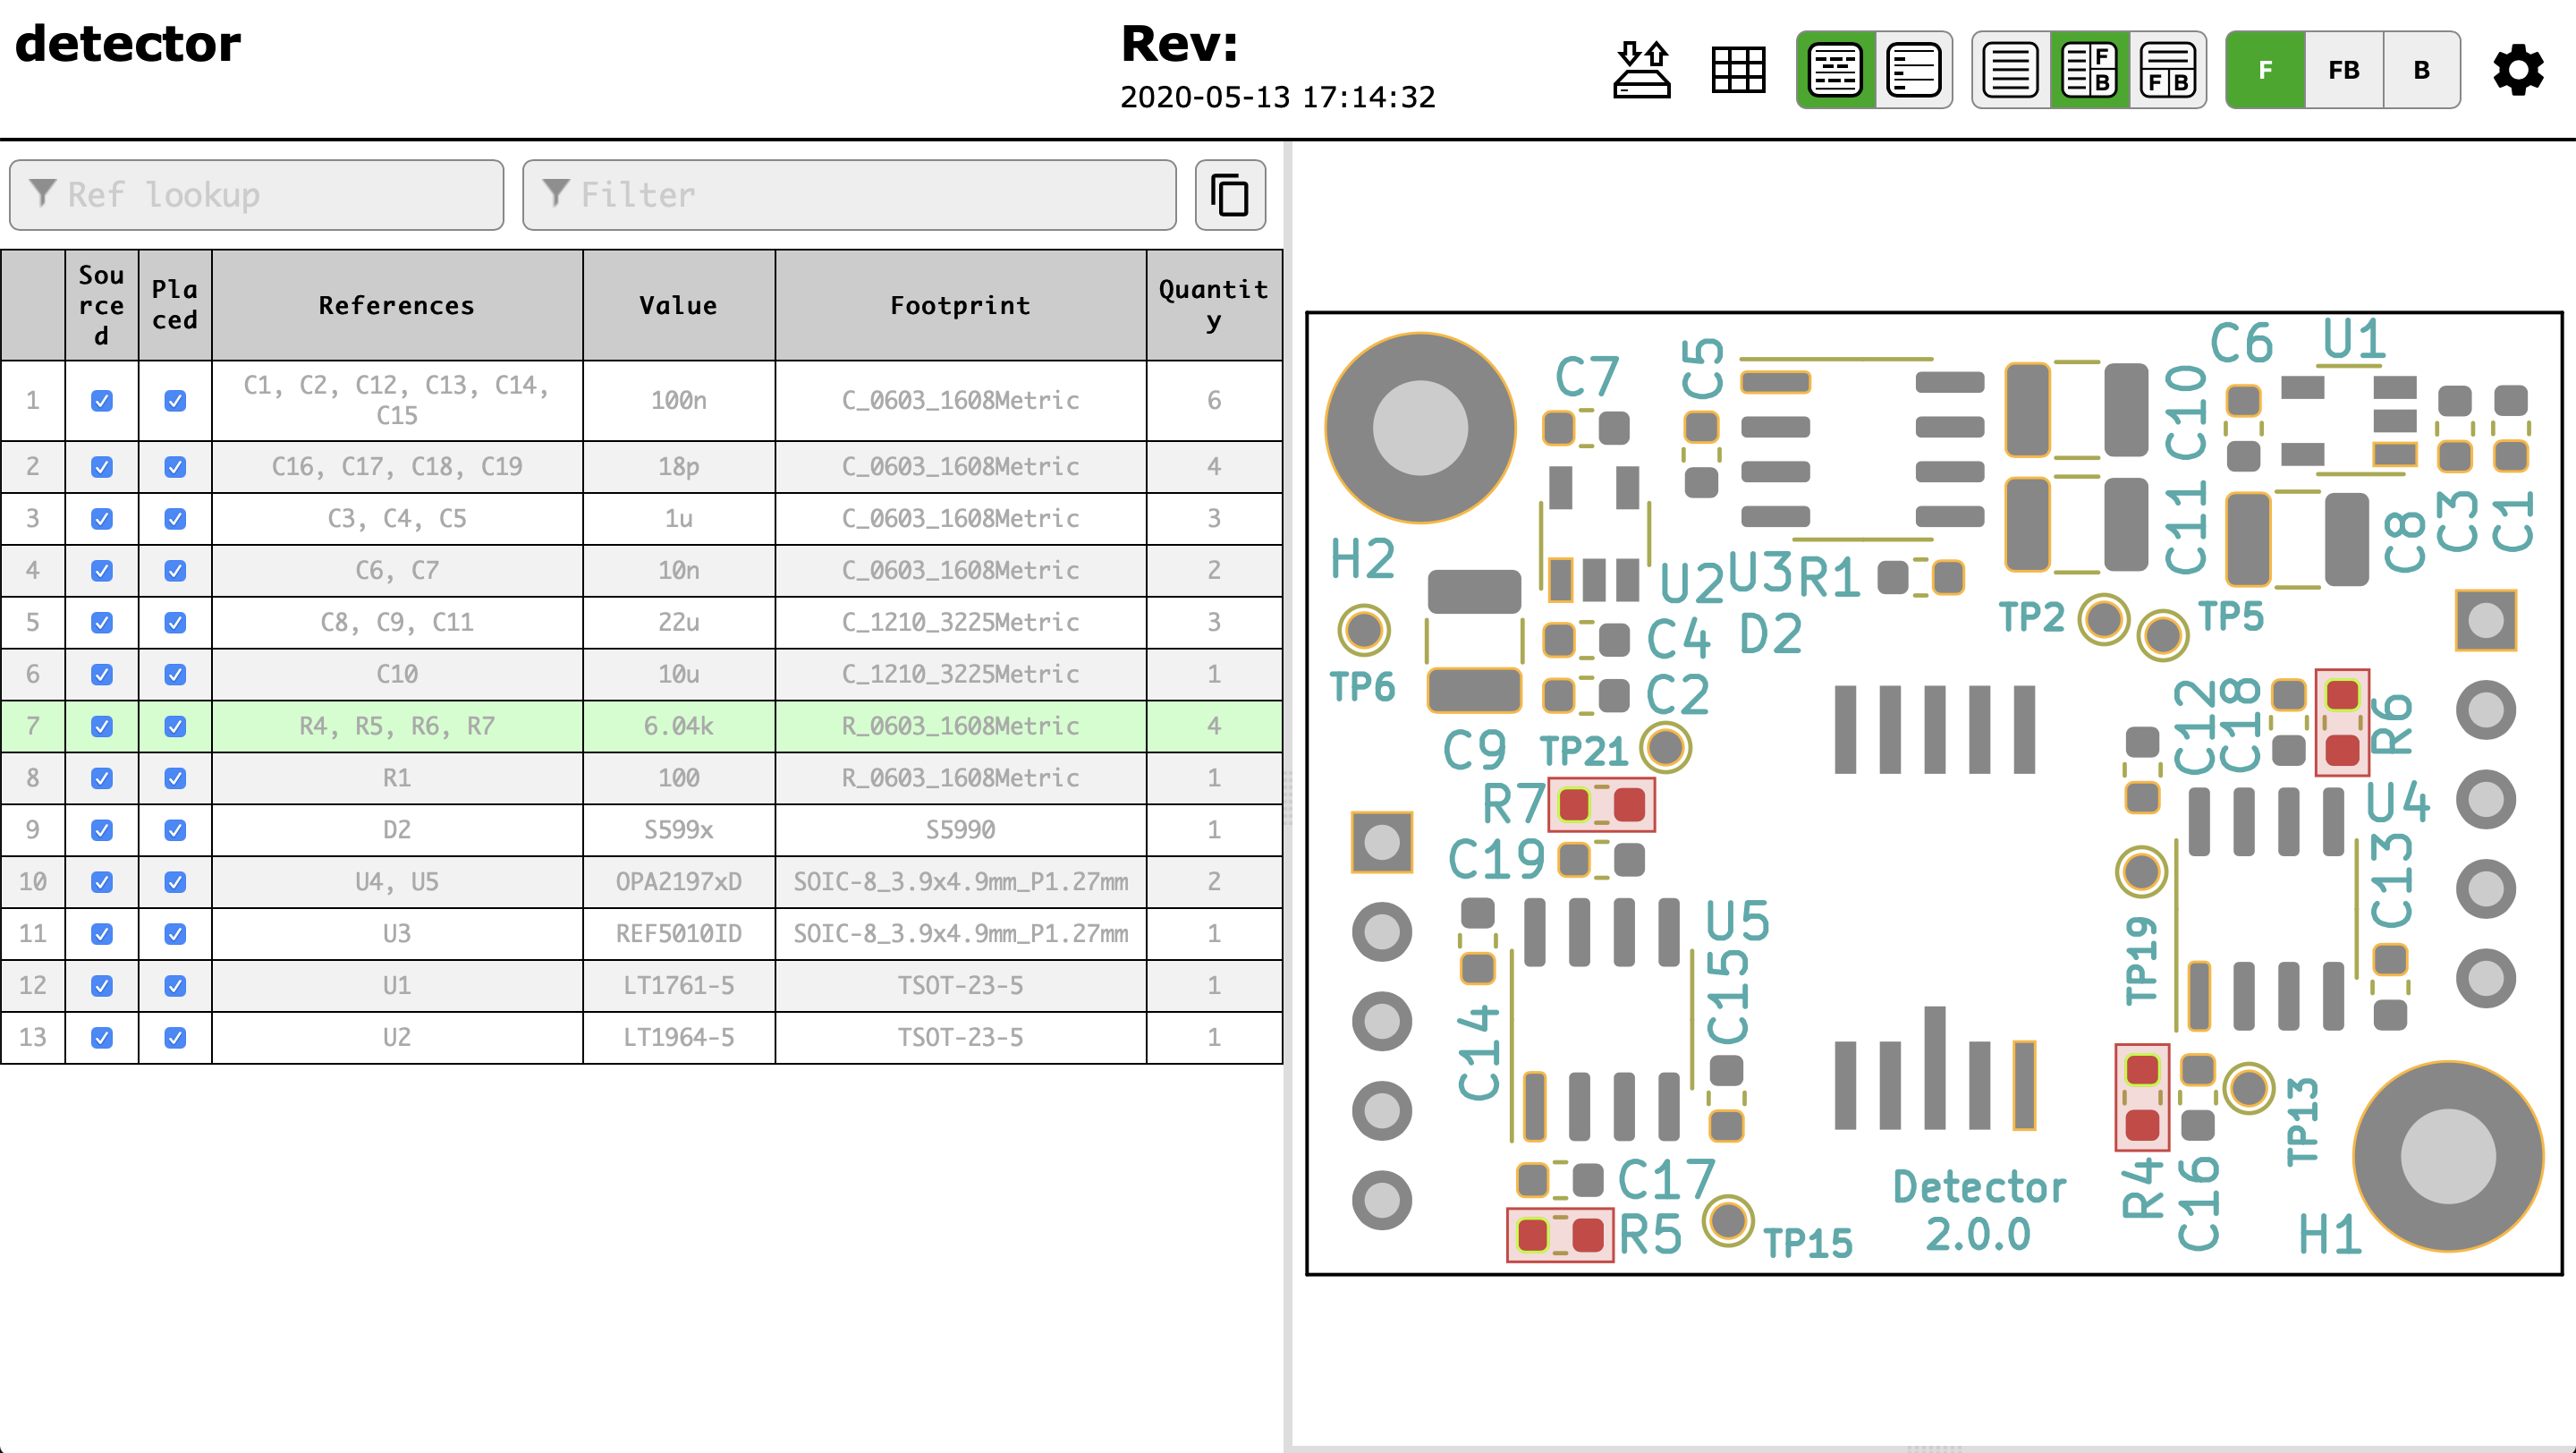
\includegraphics[scale=0.3]{screenshot/kicad_interactive_html_bom_plugin_detector}
	\caption{Detector board view of the \href{https://github.com/openscopeproject/InteractiveHtmlBom}{InteraciveHtmlBom} plugin}\label{fig:kicad_interactive_html_bom_plugin_detector}
\end{figure}
Start by checking the local inventory for the components listed by the generated \gls{html} \gls{bom}.
If certain elements are missing, you can check the \path{BOM.xlsx} file inside the project repository.
It contains part numbers and product links from major electronic distributors.
If you order, double-check with the generated \gls{html} \gls{bom}.
There might be errors, e.g., wrong casing sizes in the \path{BOM.xlsx} as it is potentially outdated.

\subsection{Manufacturing}

In the manufacturing process, we solder the components onto the PCB.
We recommend to proceed in the following steps:

\begin{enumerate}
    \item Put on rubber gloves as the solder paste is potentially hazardous.
    \item  Take out the solder paste from the fridge and let it reach room temperature\footnote{It is possible to use the cold solder paste directly, but it makes the handling more difficult as the paste is less fluid.}.
    \item Place the solder paste onto the contacts of the \gls{pcb}\footnote{Generally speaking, it is better to have too much solder paste then too less. If there is a small overlap between the contacts, this is fine as the solder will shrink when transitioning to a liquid phase in the oven.}.
    \item Place the \gls{smd} components onto the solder with a tweezer\footnote{Start with the larger components and then progress to the smaller ones}.
    \item Start the oven and adjust the frame on which you place the board with the screw to the appropriate size. Use an empty \gls{pcb} for this.
    \item Select the profile SMD180 and follow the instructions of the oven.
    \item Inspect the board for misplaced components and unmelted solder, and fix them by hand soldering\footnote{You can use the solder heat gun to melt the remaining solder paste or remove misplaced components. 
However, you might blow away small capacitors.}.
	\item Perform electrical testing as described in the next section.
	\item Solder remaining components, for example, the \gls{sma} mounts or the pin headers, by hand.
\end{enumerate}

\subsection{Electrical testing}

With the electrical testing, we want to confirm that the solder connections and components work as expected.
The most basic check is that the supply voltages are correct.
More elaborated checks concern the operational amplifiers but are out of the scope of this document.

For the arithmetic perform the following checks in the given order.
Skipping steps might lead to permanent damage!
\begin{todolist}
	\item Leave the arithmetic board unpowered and check for high resistance between the supply lines through the test points TP1 (\SI{+12}{\volt}), TP2 (GND), and TP3 (\SI{-12}{\volt})\footnote{If there is low resistance ($>\SI{10}{\kilo\ohm}$), you probably have a short through soldering.}.
	\item Configure the power supply to provide a dual voltage of \SI{\pm15}{\volt}\footnote{Alternatively, use two single voltage sources set to \SI{15}{\volt} and connect the negative port of one of the voltage sources with the other one's positive voltage.}. If possible, limit the current of the voltage sources.
	\item Confirm that the output voltages are correct with the multimeter.
	\item Connect the power supply with the arithmetic board but double-check the polarity.
	\item The voltage between TP2 and TP1 should read around \SI{+12}{\volt} while the voltage between TP2 and TP3 should read about \SI{-12}{\volt}.
	\item Confirm that the supply voltages reach the op-amps.
	\item Check the temperature of the \gls{ic}s. If any \gls{ic} is very hot, there is a short.
	\item Check if the op-amps' output voltage changes by grounding the inverting input.
\end{todolist}

For the detector perform the following checks in the given order.
Skipping steps might lead to permanent damage!
\begin{todolist}
	\item Leave the detector board unplugged and confirm high resistance between GND (you can use the middle pin of the headers), TP5 (\SI{+5}{\volt}), and TP6 (\SI{-5}{\volt}).
	\item Confirm a change of the voltage between the photodiode and GND's outer pins while illuminating the sensitive area of the photodiode with a laser pointer.
	\item Mount the detector board on the arithmetic board, and measure the detector board's supply voltages.
	\item Confirm that the voltage reference (U3) outputs \SI{10}{\volt} and that the op-amps have the correct supply voltage of \SI{\pm5}{\volt}.
\end{todolist}

Finally, we test the arithmetic amplifiers on the arithmetic board.
\begin{todolist}
	\item Mount the detector onto the arithmetic board.
	\item Measure the voltage at the outputs of the operational amplifiers of the arithmetic board. For the summing amplifier (U5), we expect an increase in voltage when illuminating the photodiode with the laser pointer.
For the difference amplifiers (U3, U4), we expect the voltage to change when moving the laser pointer's focal spot on the photodiode.
\end{todolist}
